%%
%% This is file `sample-sigconf.tex',
%% generated with the docstrip utility.
%%
%% The original source files were:
%%
%% samples.dtx  (with options: `sigconf')
%% 
%% IMPORTANT NOTICE:
%% 
%% For the copyright see the source file.
%% 
%% Any modified versions of this file must be renamed
%% with new filenames distinct from sample-sigconf.tex.
%% 
%% For distribution of the original source see the terms
%% for copying and modification in the file samples.dtx.
%% 
%% This generated file may be distributed as long as the
%% original source files, as listed above, are part of the
%% same distribution. (The sources need not necessarily be
%% in the same archive or directory.)
%%
%%%% Proceedings format for most of ACM conferences (with the exceptions listed below) and all ICPS volumes.

%%\documentclass[sigconf]{acmart}

\documentclass[acmconf,authordraft]{acmart}
%%%% As of March 2017, [siggraph] is no longer used. Please use sigconf (above) for SIGGRAPH conferences.

%%%% Proceedings format for SIGPLAN conferences 
% \documentclass[sigplan, anonymous, review]{acmart}

%%%% Proceedings format for SIGCHI conferences
% \documentclass[sigchi, review]{acmart}

%%%% To use the SIGCHI extended abstract template, please visit
% https://www.overleaf.com/read/zzzfqvkmrfzn

%%
%% \BibTeX command to typeset BibTeX logo in the docs
\AtBeginDocument{%
  \providecommand\BibTeX{{%
    \normalfont B\kern-0.5em{\scshape i\kern-0.25em b}\kern-0.8em\TeX}}}

%% Rights management information.  This information is sent to you
%% when you complete the rights form.  These commands have SAMPLE
%% values in them; it is your responsibility as an author to replace
%% the commands and values with those provided to you when you
%% complete the rights form.
\setcopyright{acmcopyright}
\copyrightyear{2018}
\acmYear{2018}
\acmDOI{10.1145/1122445.1122456}

%% These commands are for a PROCEEDINGS abstract or paper.
\acmConference[Woodstock '18]{Woodstock '18: ACM Symposium on Neural
  Gaze Detection}{June 03--05, 2018}{Woodstock, NY}
\acmBooktitle{Woodstock '18: ACM Symposium on Neural Gaze Detection,
  June 03--05, 2018, Woodstock, NY}
\acmPrice{15.00}
\acmISBN{978-1-4503-9999-9/18/06}


%%
%% Submission ID.
%% Use this when submitting an article to a sponsored event. You'll
%% receive a unique submission ID from the organizers
%% of the event, and this ID should be used as the parameter to this command.
%%\acmSubmissionID{123-A56-BU3}

%%
%% The majority of ACM publications use numbered citations and
%% references.  The command \citestyle{authoryear} switches to the
%% "author year" style.
%%
%% If you are preparing content for an event
%% sponsored by ACM SIGGRAPH, you must use the "author year" style of
%% citations and references.
%% Uncommenting
%% the next command will enable that style.
%%\citestyle{acmauthoryear}

%%
%% end of the preamble, start of the body of the document source.
\begin{document}

%%
%% The "title" command has an optional parameter,
%% allowing the author to define a "short title" to be used in page headers.
\title{Concise Description of Telecom Service Use Through Concept Chains}

%%
%% The "author" command and its associated commands are used to define
%% the authors and their affiliations.
%% Of note is the shared affiliation of the first two authors, and the
%% "authornote" and "authornotemark" commands
%% used to denote shared contribution to the research.
\author{Ants Torim}
\email{ants.torim@taltech.ee}
\author{Sadok Ben Yahia}
\email{sadok.ben@taltech.ee}
\author{Kristo Raun}
\email{kristo.raun@gmail.com}
\affiliation{%
  \institution{Tallinn University of Technology, Department of Software Science}
  \streetaddress{Akadeemia tee 15a}
  \city{Tallinn}
  \state{Estonia}
  \postcode{12618}
}





%%
%% The abstract is a short summary of the work to be presented in the
%% article.
\begin{abstract}
Binary data arise naturally in many fields including shopping carts, pass-fail tests, social networks etc. Descriptive data mining aims to discover a concise set of general patterns in these possibly noisy data. An important tool for describing binary data is Formal Concept Analysis (FCA) which describes the data through formal concepts. 
As the full lattice of formal concepts can become large even when dealing with relatively modest amounts of data  there are several methods to  reduce the number of concepts used to describe the data: selecting a subset of ``interesting''  concepts, finding a subset of  concepts that cover the data  fully etc.
In this paper we apply a novel method of concept chain coverage generation to service use data of a telecommunications company. Concept chain coverage aims to cover the data not with single concepts but with chains of related concepts. The aim is not the full coverage but high enough coverage through a concise set of concept chains. We show that a relatively modest set of concept chains (4 to 10) can describe most of the data and that the performance of the algorithm is very acceptable for this case study. 

\end{abstract}

%%
%% The code below is generated by the tool at http://dl.acm.org/ccs.cfm.
%% Please copy and paste the code instead of the example below.
%%
\begin{CCSXML}
<ccs2012>
 <concept>
  <concept_id>10010520.10010553.10010562</concept_id>
  <concept_desc>Computer systems organization~Embedded systems</concept_desc>
  <concept_significance>500</concept_significance>
 </concept>
 <concept>
  <concept_id>10010520.10010575.10010755</concept_id>
  <concept_desc>Computer systems organization~Redundancy</concept_desc>
  <concept_significance>300</concept_significance>
 </concept>
 <concept>
  <concept_id>10010520.10010553.10010554</concept_id>
  <concept_desc>Computer systems organization~Robotics</concept_desc>
  <concept_significance>100</concept_significance>
 </concept>
 <concept>
  <concept_id>10003033.10003083.10003095</concept_id>
  <concept_desc>Networks~Network reliability</concept_desc>
  <concept_significance>100</concept_significance>
 </concept>
</ccs2012>
\end{CCSXML}

\ccsdesc[500]{Computer systems organization~Embedded systems}
\ccsdesc[300]{Computer systems organization~Redundancy}
\ccsdesc{Computer systems organization~Robotics}
\ccsdesc[100]{Networks~Network reliability}

%%
%% Keywords. The author(s) should pick words that accurately describe
%% the work being presented. Separate the keywords with commas.
\keywords{big data, services, formal concept analysis, case study}

%% A "teaser" image appears between the author and affiliation
%% information and the body of the document, and typically spans the
%% page.


%%
%% This command processes the author and affiliation and title
%% information and builds the first part of the formatted document.
\maketitle

\section{Telecom Use Case}

\section{Formal Concept Analysis}
\subsection{Fundamentals of FCA}

\subsection{Concept Chains}

Concept chain is a sequence of concepts
\begin{equation}
  (C_1, C_2,..., C_n) = (\langle A_1, B_1 \rangle,\langle A_2,B_2 \rangle,  ..., \langle A_n,B_n \rangle)  \text{ ,where  }  A_i \supset  A_{i+1} \text{ for all } i
\end{equation}

Of course
\begin{displaymath}
A_i \supset A_{i+1} \equiv B_i \subset B_{i+1} \equiv C_i > C_{i+1}
\end{displaymath}

As there is an overlap between sequential extents and intents, it useful to concentrate on the differences between extents ($dA_i$) and intents ($dB_i$).

\begin{equation}
dA_k = A_k - A_{k+1}
\end{equation}

\begin{equation}
dB_k = B_k - B_{k-1}
\end{equation}

\begin{equation}
A_k = \bigcup_{i=k}^{n} dA_i
\end{equation}

\begin{equation}
B_k = \bigcup_{i=1}^{k} dB_i
\end{equation}

As there are usually too many objects to describe  individually, it is useful to replace the actual objects in the extent with the size of the extent giving us the following concept chain description:

\begin{displaymath}
 (\langle |A_1|, dB_1 \rangle,\langle |A_2|, dB_2 \rangle,  ..., \langle |A_n|, dB_n \rangle)
\end{displaymath}

\subsection{Context Coverage Problem}
\subsection{Algorithms for Generating the Concept Cover}
QualityCover

\subsection{Algorithms for Generating the Concept Chain Cover}

\section{Complete Concept Cover for Telecom Data}

\section{Concept Chain Cover for Telecom Data}

\begin{figure}[ht]
  \centering
  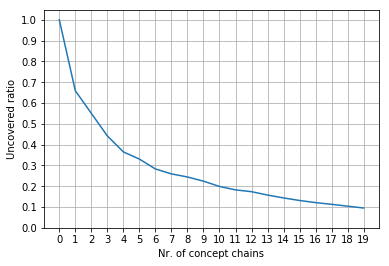
\includegraphics[width=\linewidth]{telia_ccc}
  \caption{How much of the data table is uncovered by generated concept chains.}
  \Description{Uncovered ratios.}
\end{figure}


\begin{figure}[!htb]
\vspace{.5cm}
\begin{verbatim}
service 11_______________________________411
service 56______________________316
service 18______________________315
service 64____________________297
service 44______158
service 43______157
service 65_____146
service 61__114
service 13__108
service 58_43
service 10_35
service 35_31
service 51_11
service 50_8
service 23_5
service 9_3
service 36_2
service 41_2
service 63_2
service 21_1
service 66_1
service 22_1
\end{verbatim}

\caption{First concept chain covering 34\% of the service data. $(\langle 411, service 11 \rangle,\langle 316, service 56 \rangle,  ..., \langle |A_i|, dB_i \rangle, ...)$}
\label{fig:ccc_1}
\end{figure}


\begin{figure}[!htb]
\vspace{.5cm}
\begin{verbatim}
service 35_______________________________337
service 61_________________________286
service 9___95
service 44_53
service 43_52
service 10_33
service 41_20
service 65_16
service 64_16
service 51_5
service 27_2
service 25_2
service 48_1
service 23_1
service 50_1
service 22_1
\end{verbatim}

\caption{Second concept chain covering with the first 45\% of the service data.}
\label{fig:ccc_2}
\end{figure}

\begin{figure}[!htb]
\vspace{.5cm}
\begin{verbatim}

service 13_______________________________388
service 18______________________________374
service 56______________________________374
service 21_______158
service 23_45
service 58_31
service 9_10
service 61_9
service 32_3
service 22_3
service 50_1
service 51_1
service 43_1
service 12_1
service 27_1
service 44_1
\end{verbatim}

\caption{Third concept chain covering with first and second 56\% of the service data.}
\label{fig:ccc_3}
\end{figure}


\begin{figure}[!htb]
\vspace{.5cm}
\begin{verbatim}
service 64_______________________________386
service 10___________________266
service 65________________241
service 44___119
service 43___117
service 66_18
service 48_4
service 32_3
service 21_2
service 23_2
service 26_2
service 57_2
service 45_1
service 31_1
service 34_1
\end{verbatim}

\caption{Fourth concept chain covering with first, second and third 64\% of the service data.}
\label{fig:ccc_4}
\end{figure}

\section{Conclusions}



\bibliographystyle{ACM-Reference-Format}
\bibliography{test1}

\end{document}
\endinput
%%
%% End of file `sample-sigconf.tex'.
